\chapter{Magnetostatik}\label{ms}
 \section{Grundgleichungen, Größen, Begriffe}
		  Die Magnetostatik betrachtet \textbf{zeitunabhängige} magnetische Felder soweit diese durch \textbf{Gleichströme} verursacht werden. Konstante magnetische Felder durch permanentmagnetische Stoffe werden in diesem Dokument nicht betrachtet.
		   Wesentlicher Unterschied zur Elektrostatik ist, dass es \textbf{keine magnetischen Monopole} gibt (jedenfalls keine, die nicht immer paarweise auftreten $\to$ \textbf{Spineis}). Führender Term ist also der Dipolterm.
		   Die \textbf{Grundgleichungen} sind mit \ref{GGms1} und \ref{GGms2} gegeben.
	 		Zusätzlich gilt die Materialgleichung aus \ref{matmagallg}. $\vec{B}$ und $\vec{H}$ sind i.A. nicht parallel, die Parameter sind ortsabhängig, es gibt Nichtlinearitäten und Zeitabhängikeiten ($\nearrow$\ref{mat}). Für homogene, lineare und isotrope Medien vereinfacht sich die Gleichung zu \ref{matlinhomis}. Im Vakuum gilt die selbe Gleichung (mit $\mu=\mu_0$).
	\subsection{Vektorpotential und Eichtransformation}
	\subsubsection{Begriff Vektorpotential}
		   In der Elektrostatik folgte aus $\rot \vec{E} = \vec{0}$, dass das elektrische Feld ein Gradientenfeld ist: $\vec{E} = -\grad \phi$.
		   Das ist in der Magnetostatik wegen \(\rot \vec{H}  = \vec{J} \neq \vec{0} \) nicht der Fall. Aber mit \(\div \vec{B}  = 0 \) folgt, dass \(\vec{B}  \) \textbf{quellenfrei} ist und somit als Rotation eines Vektorfeldes dargestellt werden kann ($\nearrow$\ref{poin2},\ref{helmholtz}). Das entsprechende Feld $ \vec{A}$ wird \textbf{magnetisches Vektorpotential} genannt:
		        \begin{equation}\label{magvekpot}\begin{split}
				        \boxed{\vec{B}  = \rot  \vec{A}}
			        \end{split}\end{equation}
		 Der Vorteil dieser Darstellung ist, dass $\div \vec{B}  = 0$ automatisch erfüllt ist. Im linearen und isotropen, aber \textbf{inhomogenen} Medium gilt nach \ref{matmagallg}: 
		        \begin{equation}\begin{split}
				      \vec{B}  = \mu(\vec{r} )\vec{H} \implies  \rot \vec{H}  = \rot \left( \dfrac{1}{\mu(\vec{r} )}  \vec{B}  \right) = \boxed{\rot \left( \dfrac{1}{\mu(\vec{r} )} \rot  \vec{A} \right) = \vec{J}(\vec{r} )}
			        \end{split}\end{equation}
		       Im zusätzlich homogenen Medium (\(\mu(\vec{r} ) = \mu \)) resultiert:
		        \begin{equation}\begin{split}
				        \mu \rot \vec{H}  = \rot \vec{B}  = \rot \, \rot  \vec{A} = \boxed{\grad \div  \vec{A} - \Delta  \vec{A}= \mu \vec{J}(\vec{r} )}
			        \end{split}\end{equation}
		        Der Laplace-Operator ist hier vektoriell.
  \subsubsection{Eichtransformation}\label{eichtrans}
		 Wegen $\rot \grad \psi =\vec{0}$ ist:
		        $$
			        \vec{B} ' = \rot \underbrace{\left( \vec{A} + \grad \psi\right)}_{ \vec{A}'} = \rot  \vec{A} = \vec{B}
		        $$
		  Das Vektorpotential ist folglich nur bis auf einen Summanden $\grad \psi$ bestimmt.
		  Dies kann weiter auf $\rot \, \rot  \vec{A} = \mu \vec{J}$ angewandt werden. Auch hier sieht man, dass $A'$ die Gleichung löst, wenn $A$ die Gleichung löst:
		        $$
			        \rot \, \rot  \vec{A}' = \rot \, \rot  \vec{A} = \mu \vec{J}(\vec{r} )
		        $$
		   Den Übergang
		   \begin{equation}
		    \boxed{ \vec{A}' =  \vec{A} + \grad \psi}
		    \end{equation}
		     nennt man \textbf{Eichtransformation} ($\nearrow$\ref{geneich}). Da $\vec{B} '=\vec{B} $ gilt, heißt die magnetische Flussdichte \textbf{eichinvariant}. Für die Divergenz gilt:
		        $$
			        \div  \vec{A}' = \div \left( \vec{A} + \grad \psi \right) = \underbrace{\div \vec{A}}_{=0\nearrow\text{\ref{divrot}}}  + \underbrace{\div \grad \psi}_{\ne 0}
		        $$
		    Man kann erkennen, dass die Divergenz von $A'$ eine andere ist, als die Divergenz von $A$, obwohl $B$ bei $A$ und $A'$ gleich ist. In ${\grad \textcolor{red}{\div  \vec{A}} - \Delta  \vec{A}= \mu \vec{J}(\vec{r} )}$ kann $\div  \vec{A}$ also \textbf{beliebig} (aber physikalisch sinnvoll, mathematisch muss ein $\psi$ gefunden werden können, sodass $\div\vec{A}=\Delta \psi$ gilt) gewählt werden, ohne dabei das resultierende $\vec{B}$ zu verändern. Für statische Probleme ist die \textbf{Coulomb-Eichung} ($\nearrow$\ref{couleich}) gut geeignet:
			        \begin{equation}\label{vektorpot}
			        	    \boxed{\div  \vec{A} = 0} \quad \implies \quad \boxed{\Delta  \vec{A}= -\mu \vec{J}(\vec{r} )}
			        \end{equation}			        
			   \textbf{Achtung:} Der Laplace-Operator $\Delta $ für Vektorfelder muss im allgemeinen Fall (krummlinige Koordinaten) aus der Beziehung $\Delta \cdot = \grad \, \div \cdot - \rot \, \rot \cdot$ ausgerechnet werden, bzw. muss eine Produktregel angewandt werden ($\nearrow$ \ref{laplaceop}). Hierbei \enquote{vermischen} sich die Komponenten wegen der Ortsabhängigkeit der Einheitsvektoren. \textbf{Nur für kartesische Koordinaten} zerfällt die vektorielle Poissongleichung in drei skalare Poissongleichungen:
			        \begin{equation}\begin{split}
					        & \Delta  A _\mathrm{x} = -\mu  J_\mathrm{x}\\
					        & \Delta  A _\mathrm{y} = -\mu  J_\mathrm{y}\\
					        & \Delta  A _\mathrm{z} = -\mu  J_\mathrm{z} \text{ mit} \\
					        &  \vec{A} =  A _\mathrm{x}  \vu{x} +  A _\mathrm{y}  \vu{y} +  A _\mathrm{z}  \vu{z}\\
					        & \vec{J} = J_\mathrm{x}  \vu{x} + J_\mathrm{y}  \vu{y} + J_\mathrm{z}  \vu{z} \\
					        &\Delta = \dfrac{\partial^2}{\partial x^2} + \dfrac{\partial^2}{\partial y^2} + \dfrac{\partial^2}{\partial z^2} \text{ (skalarer Laplace-Operator)}
				        \end{split}\end{equation}
			   z.B. in Zylinderkoordinaten (\(\rho,\,\varphi,\,z \)) ergibt sich
			        \begin{equation}\begin{split}
					        \Delta  A _{\rho} - \dfrac{2}{\rho^2} \dfrac{\partial  A _{\varphi}}{\partial \varphi} - \dfrac{ A _{\rho}}{\rho^2} &= -\mu J_{\rho} \\
					        \Delta  A _{\varphi} + \dfrac{2}{\rho^2}  \dfrac{\partial  A _{\rho}}{\partial \varphi} - \dfrac{ A _{\varphi}}{\rho^2} &= -\mu J_{\varphi} \\
					        \Delta  A _\mathrm{z} &= -\mu  J_\mathrm{z}
				        \end{split}\end{equation}
			        mit
			        \begin{equation}
				        \Delta = \dfrac{1}{\rho} \dfrac{\partial}{\partial \rho} \rho \dfrac{\partial}{\partial \rho} + \dfrac{1}{\rho^2} \dfrac{\partial^2}{\partial \varphi^2} + \dfrac{\partial^2}{\partial z^2} \text{ (skalarer Laplace-Operator)}
			        \end{equation}
			        Insbesondere sieht man hier, dass die Laplace-Gleichung für den Vektor $\vec{A}$ nicht den Laplace-Gleichungen für die Komponenten $A_\varphi$ und $A_\varrho$ entspricht, wie es kartesisch der Fall wäre. Während man im kartesischen Fall die Projektion auf die Einheitsvektoren in den Laplace-Operator hineinziehen kann, geht das im Fall nicht konstanter Einheitsvektoren nicht.
  \subsection{Berechnung des Vektorpotentials und der Flussdichte}
  \subsubsection{Vektorpotential}
		  Für den Fall \textbf{kartesischer Koordinaten} ergeben sich drei Poisson-Gleichungen (offensichtlich nicht für Zylinderkoordinaten). Es sind also die in der Elektrostatik behandelten Lösungsmethoden ($\nearrow$\ref{poilsg}) anwendbar.  Analog zu \ref{PotR} ergibt sich
		        \begin{equation}\begin{split}
				        &  A _\mathrm{x}(\vec{r} ) = \dfrac{\mu}{4 \pi} \iiint\limits_{V} \dfrac{J_\mathrm{x}(\vec{r}' ) }{\left| \vec{r}  - \vec{r}'  \right|} \dd V' \\
				        &  A _\mathrm{y}(\vec{r} ) = \dfrac{\mu}{4 \pi} \iiint\limits_{V} \dfrac{J_\mathrm{y}(\vec{r}' ) }{\left| \vec{r}  - \vec{r}'  \right|} \dd V' \\
				        &  A _\mathrm{z}(\vec{r} ) = \dfrac{\mu}{4 \pi} \iiint\limits_{V} \dfrac{J_\mathrm{z}(\vec{r}' ) }{\left| \vec{r}  - \vec{r}'  \right|} \dd V'
			        \end{split}\end{equation}
		         Das Ergebnis ist eine partikuläre Lösung der Poisson-Gleichung und lässt sich wieder \textbf{koordinatenfrei} schreiben (dieses Ergebnis stimmt für beliebige Koordinaten):
		        \begin{equation} \label{Akoordfrei}
			        \boxed{ \vec{A}(\vec{r} ) = \dfrac{\mu}{4 \pi} \iiint\limits_{V} \dfrac{\vec{J}(\vec{r}' )}{\left| \vec{r}  - \vec{r}'  \right|} \dd V'}
		        \end{equation}
		  Für einen \textbf{Stromfaden} (Draht) folgt der Spezialfall (Aufteilung der Integration auf Querschnittsfläche und Linienintegral entlang des Stromfadens)
		        \begin{equation}\label{Astromfad}
			       \boxed{ \vec{A}(\vec{r} ) = \dfrac{\mu}{4  \pi}   I  \oint\limits_{C} \dfrac{\dd \vec{r}'}{\left| \vec{r}  - \vec{r}'  \right|}}
		        \end{equation}
  \subsubsection{Berechnung der magnetischen Flussdichte - Gesetz von Biot-Savart}
		   Mit \ref{magvekpot} und \ref{Akoordfrei} folgt
		        $$
			        \vec{B} (\vec{r} ) = \dfrac{\mu}{4 \pi} \iiint\limits_{V} \rot _\mathrm{r} \dfrac{\vec{J}(\vec{r}' )}{\left| \vec{r}  - \vec{r}'  \right|} \dd V'
		        $$
		   Man berechnet
		        \begin{equation}\begin{split}
				        \rot _\mathrm{r} \dfrac{\vec{J}(\vec{r}' )}{\left| \vec{r}  - \vec{r}'  \right|} &= \dfrac{1}{\left| \vec{r}  - \vec{r}'  \right|}  \cancelto{0}{\rot _\mathrm{r} \vec{J}(\vec{r}' )} - \vec{J}(\vec{r}' ) \times \grad _\mathrm{r} \dfrac{1}{\left| \vec{r}  - \vec{r}'  \right|} \\
				        &= -\vec{J}(\vec{r}' ) \times \grad _\mathrm{r} \dfrac{1}{\left| \vec{r}  - \vec{r}'  \right|} = -\vec{J}(\vec{r}' ) \times \left( -\dfrac{\left( \vec{r}  - \vec{r}'  \right)}{\left| \vec{r}  - \vec{r}'  \right|^3} \right) = \vec{J}(\vec{r}' ) \times \dfrac{\vec{r}  - \vec{r}' }{\left| \vec{r}  - \vec{r}'  \right|^3}
			        \end{split}\end{equation}
		   Damit folgt das das allgemeine \textbf{Biot-Savart-Gesetz}:
		        \begin{equation}\label{biot-savart}
			        \boxed{\vec{B} (\vec{r} ) = \dfrac{\mu}{4  \pi} \iiint\limits_{V} \dfrac{\vec{J}(\vec{r}' ) \times \left( \vec{r}  - \vec{r}'  \right)}{\left| \vec{r}  - \vec{r}'  \right|^3} \dd V'}
		        \end{equation}
		  Für Stromfäden folgt:
		        \begin{equation}
			        \boxed{\vec{B} (\vec{r} ) = -\dfrac{\mu}{4  \pi}   I  \oint\limits_{C} \dfrac{\left( \vec{r}  - \vec{r}'  \right) \times \dd \vec{r}'}{\left| \vec{r}  - \vec{r}'  \right|^3}} 
		        \end{equation}	
  \subsection{Energie im magnetostatischen Feld}
		   Analog zur Elektrostatik erhält man für die \textbf{magnetische Energiedichte}:
		        \begin{equation}\label{edichteH}
			        \boxed{  w _\mathrm{m} = \dfrac{1}{2} \cdot \vec{H}  \cdot \vec{B} }
		        \end{equation}
		   Für die gesamte \textbf{magnetische Energie}:
		        \begin{equation}
			        \boxed{ W _\mathrm{m} = \dfrac{1}{2} \cdot \iiint\limits_{V} \vec{H}  \cdot \vec{B}  \dd V}
		        \end{equation}
		    Für lineare, homogene und isotrope Medien gilt:
		        \begin{align*}
			       & & W _\mathrm{m} &= \dfrac{1}{2 \mu} \cdot \iiint\limits_{V} \vec{B} ^2 \dd V\\
				        \text{mit}&& \div \left(  \vec{A} \times \vec{B}  \right) &= \vec{B}  \cdot \underbrace{\rot  \vec{A}}_{\vec{B} } -  \vec{A} \cdot \underbrace{\rot \vec{B} }_{\mu \vec{J}} \\
				        &&&= \vec{B} ^2 - \mu   \vec{A} \cdot \vec{J}\\
			       				      \implies&&  W _\mathrm{m} &= \dfrac{1}{2}  \iiint\limits_{V}  \vec{A} \cdot \vec{J} \dd V + \dfrac{1}{2 \mu} \cdot \iiint\limits_{V} \div \left(  \vec{A} \times \vec{B}  \right) \dd V\\
				       && &= \dfrac{1}{2}\iiint\limits_{V}  \vec{A} \cdot \vec{J} \dd V + \dfrac{1}{2 \mu} \oiint\limits_{O(V)}  \vec{A} \times \vec{B}  \cdot \dd\vec{F}
			        \end{align*}
		    Aus Biot-Savart folgt \(\left| \vec{B}  \right| \sim r^{-2} \) bei einer \textbf{endlich ausgedehnten Stromverteilung}.  Weiterhin ist in diesem Fall \(\left|  \vec{A} \right| \sim r^{-1} \), sodass \( \vec{A} \times \vec{B}  \sim r^{-3} \) gilt. Integriert man über den kompletten Raum, dann ist das Oberflächenintegral $\iiint\limits_{O(V)}...$ folglich null (die Fläche wächst nur $\sim r^2$). Das Volumenintegral muss in allen Bereichen ausgewertet werden, in denen $J\neq 0$:
		        \begin{equation}\begin{split}
				          \Aboxed{W _\mathrm{m}& = \dfrac{1}{2} \cdot \iiint\limits_{V}  \vec{A} \cdot \vec{J} \dd V}\\
				          \Aboxed{ w _\mathrm{m}& = \dfrac{1}{2} \cdot  \vec{A} \cdot \vec{J} }
			        \end{split}\end{equation}
  \subsection{Induktivität}
	  \begin{center}
		  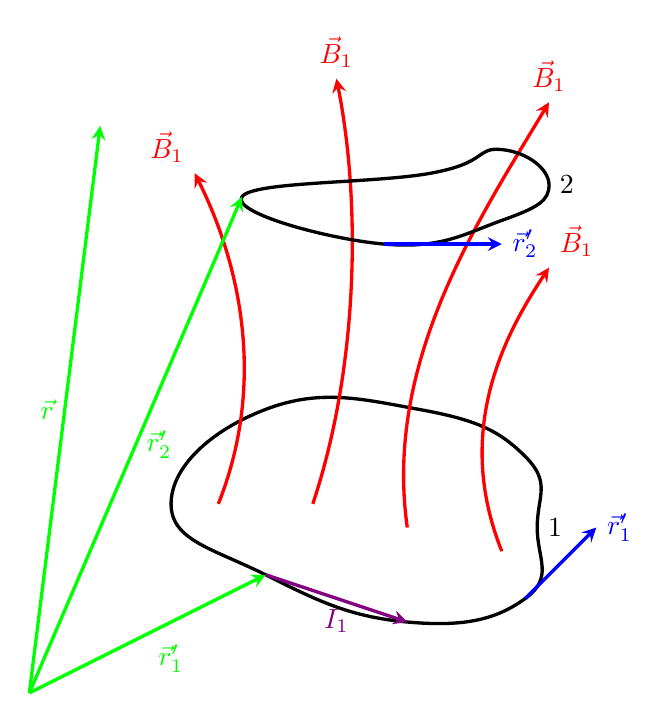
\begin{tikzpicture}[line width = 1.2pt, line join=round,x=1cm,y=1cm,>=stealth, scale = 3]
	% Schleife 1
	\coordinate (a) at (1,0.5);
	\coordinate (b) at (1.6,0.3);
	\coordinate (c) at (2.1,0.4);
	\draw plot [smooth cycle, tension=0.8] coordinates {(2.1,1) (1.65,1.2) (1,1.2) (0.6,0.8) (a) (b) (c) (2.15,0.7)} node [anchor=west] {$ 1 $};
	% Strom 1
	\draw [->, color=violet] (a) -- (b) node [anchor = north,midway] {$  I_1 $};
	% differentieller Weg 1
	\draw [->, color = blue]  (c) -- ++(0.3,0.3) node[anchor=west] { $ \dd  \vec{r}'_1 $ };
	% magnetische Flussdichte
	\draw [->,color=red] (0.8,0.8) .. controls (1,1.3) and (0.9,1.8) .. (0.7,2.2) node[anchor=south east]{$ \vec{B} _1 $};
	\draw [->,color=red] (1.2,0.8) .. controls (1.4,1.4) and (1.4,2.1) .. (1.3,2.6) node[anchor=south]{$ \vec{B} _1 $};
	\draw [->,color=red] (1.6,0.7) .. controls (1.5,1.4) and (1.9,2) .. (2.2,2.5) node[anchor=south]{$ \vec{B} _1 $};
	\draw [->,color=red] (2,0.6) .. controls (1.8,1.1) and (2,1.5) .. (2.2,1.8) node[anchor=south west]{$ \vec{B} _1 $};
	% Schleife 2
	\coordinate (ab) at (1.5,1.9);
	\coordinate (bb) at (0.9,2.1);
	\draw plot [smooth cycle, tension=0.8] coordinates {(2,2.3) (1.7,2.2) (bb) (ab) (2,2) (2.2,2.15) } node[anchor=west]{$ 2 $};
	% differentieller Weg 2
	\draw [->,color=blue] (ab) -- ++(0.5,0) node[anchor = west] { $ \dd  \vec{r}'_2 $ };
	% Ortsvektoren
	\draw [->,color=green] (0,0) -- (a) node[anchor=north west,midway] {$ \vec{r}' _1 $};
	\draw [->,color=green] (0,0) -- (bb) node[anchor=west,midway] {$ \vec{r}' _2 $};
	\draw [->,color=green] (0,0) -- (0.3,2.4) node[anchor=east,midway] {$ \vec{r}  $};
\end{tikzpicture}
	  \end{center}
		   In der Schleife 1 fließt der Strom \( I_1 \). Nach Biot-Savart gilt also:
		        \begin{equation}
			        \vec{B} _1 = -\dfrac{\mu_0}{4 \pi} I_1 \oint\limits_{C_1} \dfrac{\left( \vec{r}  - \vec{r}' _1 \right) \times \dd \vec{r}'_1}{\left| \vec{r}  - \vec{r}' _1 \right|^3}
		        \end{equation}
		   Der magnetische Fluss (in der zweiten Schleife hervorgerufen durch den Strom in der ersten Schleife) $\phi_{m,21}$ durch die Schleife 2 ist demnach:
		        \begin{equation}\label{fluss1}
			        \phi_{m,21} = \iint\limits_{F_2} \vec{B} _1 \cdot \dd\vec{F}_2, \quad \left| \vec{B} _1 \right| = B_1 \sim  I_1
		        \end{equation}
		   Mit der Gleichung 
		   \begin{equation} \label{gegeninddef}
		  \boxed{\phi_{m,21} = M_{21}  I_1}
	\end{equation} wird $ M_{21}$ als \textbf{Gegeninduktivität} definiert. Um eine Berechnungsvorschrift für $ M_{21}$ zu erhalten, wird \ref{fluss1} näher betrachtet  (\(\vec{r}' _2 \) liegt auf \(C_2 \)):
	  \begin{equation}
		  \phi_{m,2} = \iint\limits_{F_2} \vec{B} _1 \cdot \dd\vec{F}_2 = \iint\limits_{F_2} \rot  \vec{A}_1 \cdot \dd\vec{F}_2 \stackrel{\text{\ref{stokes}}}{=} \oint\limits_{C_2}  \vec{A}_1 \cdot \dd\vec{r}'_2 \stackrel{\text{\ref{Astromfad}}}{=} \dfrac{\mu_0}{4 \pi}   I_1 \oint\limits_{C_2} \oint\limits_{C_1} \dfrac{\dd  \vec{r}'_1}{\left| \vec{r}' _2 - \vec{r}' _1 \right|} \cdot \dd\vec{r}'_2
	  \end{equation}
		Durch Koeffizientenvergleich mit \ref{gegeninddef} folgt eine Formel für die Gegeninduktivität:
		        \begin{equation}
		        \boxed{ M_{21} = \dfrac{\mu_0}{4 \pi}  \oint\limits_{C_2} \oint\limits_{C_1} \dfrac{\dd  \vec{r}'_1 \cdot \dd \vec{r}'_2}{\left| \vec{r}' _2 - \vec{r}' _1 \right|} } 
		        \end{equation}
		   Diese Formel wird \textbf{Neumann-Formel} genannt, ist aber nicht besonders nützlich zur Berechnung von \( M_{21} \). Dennoch können aus ihr wichtige Eigenschaften abgelesen werden:
		        \begin{enumerate}
			        \item \( M_{21} =  M_{12} =  M \) 
			        \item \( M_{21} \) ist zunächst eine rein geometrische Größe, in der Berechnung von $M$ kommen nur Konstanten und geometrische Parameter vor. Erst wenn Ursache und Wirkung mit Richtungssinn bekannt sind, kann man $M$ vorzeichenbehaftet interpretieren (bspw. können Spulen gleich- oder gegensinnig gekoppelt sein, was im Vorzeichen von $M$ berücksichtigt werden kann $\nearrow$ EMF).
		        \end{enumerate}
		   Wenn \(C_1 = C_2 \) ist, dann ist die Neumann-Formel so nicht anwendbar (Singularitäten, da $\vec{r}' _2 = \vec{r}' _1$). Der Fluss in der Leiterschleife 1 hervorgerufen durch den Strom in der Leiterschleife 1 berechnet sich durch:
		        \begin{equation}
			        \phi_{m,11} =  M_{11} \cdot  I_1 \xrightarrow{\text{umbenennen}} \boxed{\phi_{m,11} =  L_1 \cdot  I_1 } 
		        \end{equation}
		    Dabei ist $L$ die \textbf{Selbstinduktivität}. Durch Koeffizientenvergleich erhält man auch für diese eine Berechnungsvorschrift:
		        \begin{equation}\begin{split}
			        \phi_{m,11} &= \iint\limits_{F_1} \vec{B}_1  \cdot \dd\vec{F}_1 = \oint\limits_{C_1}  \vec{A}_1 \cdot \dd\vec{r}'_1  \stackrel{!}{=}  L_1  I_1 \\
			        \implies 	\Aboxed{ L_i &= \dfrac{1}{ I_i}\oint\limits_{C_i}  \vec{A_i} \cdot \dd\vec{r}'_i}
		        \end{split}\end{equation}
		   Für die magnetische Energie folgt für lineare, homogene und isotrope Medien (durch Zerlegung des Volumenintegrals in ein Flächen- und ein Wegintegral):
		        \begin{equation}
			        W _\mathrm{m} = \dfrac{1}{2}  \iiint\limits_{V}  \vec{A} \cdot \vec{J} \dd V
			        = \dfrac{1}{2}  I \underbrace{\oint\limits_{C}  \vec{A} \cdot \dd\vec{r}'}_{= L  I} = \dfrac{1}{2}  L  I^2
		        \end{equation}
		        Der Fall, dass beide Schleifen von einem Strom durchflossen sind oder die Schleifen mehrfach gewickelt sind (Windungszahl $w>1$) wurde in $\nearrow$ EMF Kapitel 5 betrachtet. Es ist zu beachten, dass dort das dynamische Magnetfeld behandelt wurde, während sich \textbf{hier} zunächst auf den \textbf{statischen Fall} beschränkt wird.
  \subsection{Magnetisches Moment}
		   Das Vektorpotential aus \ref{Akoordfrei} wird nun für den Fall von {großer Entfernung des Beobachtungspunktes zu der lokal beschränkten Stromdichte} untersucht. Dies läuft auf eine \textbf{Multipolentwicklung} hinaus, in großer Entfernung dominiert hier der Dipolterm, da der Monopolterm verschwindet (keine magnetischen Monopole). Setzt man \ref{Taylrrr} in das Integral ein, so gilt zunächst:
		   \begin{equation}
		   \vec{A}(\vec{r} ) = \frac{\mu}{4 \pi} \frac{1}{r}\iiint\limits_{V} \vec{J}(\vec{r}' ) \dd V'  + \frac{\mu}{4 \pi} \frac{1}{r^3}\iiint\limits_{V} \vec{r} \cdot \vec{r}'  \vec{J}(\vec{r}' ) \dd V' + \dots
		   \end{equation}
		    Damit folgt (Monopolterm verschwindet):
		         \begin{equation}
			        \vec{A}(\vec{r} ) = \frac{\mu}{4 \pi} \frac{1}{r^3}\iiint\limits_{V}\vec{r} \cdot \vec{r}'   \vec{J}(\vec{r}' ) \dd V' + \dots = \frac{\mu}{4 \pi} \underbrace{\frac{1}{2}\iiint\limits_{V} \vec{r}'  \times \vec{J}(\vec{r}' ) \dd V'}_{\vec{m}(\vec{r} )}  \times \frac{\vec{r} }{r^3}  + \dots
		        \end{equation}
		   Mit dem \textbf{magnetischem Moment} $\vec{m}$ ist das Vektorpotential somit:
		        \begin{equation}
			        \boxed{ \vec{A}(\vec{r} ) = \frac{\mu}{4 \pi} \frac{\vec{m}(\vec{r} )  \times \vec{r} }{r^3}  + \dots} \to \boxed{\vec{B} (\vec{r} ) = \frac{\mu}{4 \pi} \left[ \frac{3(\vec{r} \cdot \vec{m}(\vec{r} )) \vec{r}  }{r^5} -\frac{\vec{m}(\vec{r} )}{r^3}\right] + \dots}
		       \end{equation}

 \section{Materie}\label{magmaterial}
		  Wie bereits in \ref{materie} erwähnt wurde, gelten die Maxwell-Gleichungen des Vakuums ($\nearrow$\ref{mikrosmax}) \textbf{unverändert} in Materie. Allerdings müssten dann die \textbf{Bewegungen aller Ladungsträger} betrachtet werden, die aber nur zu einem Bruchteil zu einer \textbf{makroskopischen Stromdichte} beitragen. Analog der Elektrostatik bietet es sich an, eine makroskopische Betrachtung im Sinne von Mittelwerten anzustreben ($\nearrow$\ref{makrmax}).
		  \subsection{Makroskopische Größen}
		  Analog zum elektrischen Fall ($\nearrow$ \ref{DEMat}, in \ref{elmaterial} wird beispielhaft eine Vereinfachung der komplizierten Zusammenhänge ausgeführt) wird die Materialabhängigkeit der \textbf{Magnetisierung} $\vec M$ durch einen Parameter $\zeta_\mathrm m$ beschrieben. Wieder vereinfacht sich der Zusammenhang in der Näherung $\vec M=\frac{1}{\mu_0}\zeta_\mathrm m\vec B$.
		  Eingesetzt ergibt das:
		  \begin{equation}\vec{H}=\frac{1}{\mu_0}\vec{B}-\vec{M}=\frac{1}{\mu_0}\underbrace{\left( 1-\zeta_{\mathrm m} \right)}_{1/\mu_r}\vec{B}=\frac{1}{\mu_0\mu_r}\vec{B}=\frac{1}{\mu}\vec{B}\end{equation}
		  Historisch bedingt wird $\zeta$ durch $\chi$ ersetzt, es gilt $(1-\zeta_\mathrm m)\cdot (1+\chi_\mathrm m)=1$. Für kleine Werte gilt $\zeta_\mathrm m \approx \chi_\mathrm m$. Damit folgt:
		        \begin{align}\label{matmagallg}
			         & \boxed{\vec{H}  = \dfrac{1}{\mu_0} \vec{B}  - \vec{M}}
			         &                                                        & \Leftrightarrow
			         &                                                        & \boxed{\vec{B}  = \mu_0  \left( \vec{H}  + \vec{M} \right)}
		        \end{align}
		  In der Maxwellgleichung \ref{GGms1} ist $\vec{J}$ dann als \textbf{makroskopisch gemittelte Stromdichte} zu verstehen. Für ein \textbf{lineares und isotropes Medium} (vgl. \ref{elmaterial}) kann mit Hilfe der \textbf{magnetischen Suszeptibilität} \(\chi_\mathrm{m} \) (in homogenen Medien ortsunabhäniger Skalar) analog \ref{elsus} geschrieben werden:
		  \begin{equation}
		  	{\vec{M} = \chi_\mathrm{m}  \vec{H} }
		  \end{equation}
		  Somit ergibt sich für die magnetische Flussdichte analog \ref{susversch}:
		        \begin{equation}\label{magsus}\boxed{\vec{B}  = \left( 1 + \chi_\mathrm{m} \right) \mu_0 \vec{H} = \mu_0 \mu_\mathrm{r} \vec{H}  }\end{equation}
Die Größe ${\mu_\mathrm{r} = 1 + \chi_\mathrm{m} }$ ist die \textbf{Permeabilitätszahl} (relative Permeabilität).
  \subsection{Typen von magnetischer Materie}
		   \subsubsection{Diamagnetismus}
			         Diamagnetismus ist eine Eigenschaft \textbf{aller Stoffe}, kann aber von stärkeren anderen Eigenschaften überlagert werden. Im Fall von (nur) Diamagnetismus hat man keine permanenten internen magnetische Dipole. Daher gibt es nur eine induzierte Magnetisierung durch das äußere Feld, welche ihrer Ursache entgegen wirkt. Es gilt $\chi_\mathrm{m} < 0$ und $|\chi_\mathrm{m}| \simeq 10^{-5}$.
			         Ein Spezialfall des Diamagnetismus ist der Meißner-Ochsenfeld-Effekt in \textbf{Supraleitern} (komplette Feldverdrängung), hier ist
			              $\chi_\mathrm{m} = -1\implies \mu_r=0$, was auch als perfekter Diamagnetismus bezeichnet wird.
		  \subsubsection{Paramagnetismus}
			         Es gibt \textbf{permanente interne magnetische Dipole}, die sich im äußeren Feld orientieren können. Die thermische Bewegung wirkt der Ordnung entgegen. Daher gilt allgemein: $\chi_\mathrm{m} > 0 \text{ und } \chi_\mathrm{m} = \chi_\mathrm{m}(T)$. Je nach Ursache des Paramagnetismus (gebundene Elektronen vs. freie Leitungselektronen) ist die magnetische Suszeptibilität entweder \textbf{temperaturabhängig} (gebundene Elektronen) oder (fast) \textbf{temperaturunabhängig} (Leitungselektronen $\to$ \textbf{Pauli-Paramagnetismus}).
			         Im Falle der Temperaturabhängigkeit gilt (zumindest bei ausreichend hohen Temperaturen) das \textbf{Curie-Gesetz} $\chi_\mathrm{m}(T) = \frac{C}{T}$.
		  \subsubsection{Kollektiver Magnetismus} 
		  Es gibt \textbf{permanente interne magnetische Dipole}, die sich im äußeren Feld orientieren können. Die thermische Bewegung wirkt der Ordnung entgegen. Unterhalb einer kritischen Temperatur $T^\star$ kommt es aber durch eine (quantenmechanische) \textbf{Austauschwechselwirkung} auch ohne äußeres Feld zu einer \textbf{spontanen Ausrichtung}. Die Suszeptibilität ist häufig eine komplizierte Funktion (mindestens) von Feld und Temperatur:
			              $
				              \chi_\mathrm{m} = \chi_\mathrm{m}(T, H, \dots)
			              $.
			         Der kollektive Magnetismus gliedert sich in Ferro-, Ferri- und Antiferromagnetismus. \\\\
	  \textbf{Ferromagnetismus} (teilweise basierend auf \href{https://de.wikipedia.org/wiki/Ferromagnetismus}{Wikipedia})\textbf{:}\\
	   Wichtige Stoffe sind Fe, Co und Ni. Man unterscheidet die folgenden Temperaturbereiche:
	   \begin{itemize}
	   	\item $T=0$: Alle permanenten magnetischen Dipole sind gleich ausgerichtet.
	   	\item $0<T\le T^\star=T_C$ \textbf{(Curie-Temperatur)}: zunehmende Unordnung durch thermische Bewegung
	   	\item $T>T_C$: normaler Paramagnetismus
	   \end{itemize}
Ferromagnetische Stoffe haben ein $\chi_m > 0$ mit $|\chi_m|\gg 1$. Es gibt eine \textbf{Hysterese}. Die Ursache für das Verhalten sind die sogenannten \textbf{Weiss-Bezirke}. Sie zeichnen sich dadurch aus, dass die Spins der Elektronen, die als Elementarmagnete aufgefasst werden können, innerhalb eines Bezirks parallel zueinander sind. Die Grenzen zwischen den Bezirken heißen \textbf{Bloch-Wände}. Wird nun ein äußeres Magnetfeld angelegt, so wachsen die Bezirke, deren Orientierung der Ausrichtung des Magnetfeldes entspricht, auf Kosten der anderen Bezirke, indem Elektronen in den anderen Bezirken \enquote{umklappen}, sich also parallel zum Magnetfeld ausrichten. Anschaulich entspricht das einer Verschiebung der Bloch-Wände.\\
Störstellen, die in jedem Ferromagnetikum existieren, (in Eisen z. B. Kohlenstoffeinschlüsse) verhindern jedoch, dass das Verschieben der Bloch-Wände gleichmäßig verläuft. Wenn eine Bloch-Wand beim Verschieben auf eine Störstelle trifft, so bleibt sie zuerst an ihr hängen, und es bildet sich hinter der Störstelle eine Art Blase, in der die Spins der Elektronen noch nicht umklappen. Erst ab einer bestimmten Feldstärke schließt sich diese Blase, was zu einer plötzlichen Änderung der Magnetisierung führt. Dieser Vorgang wird \textbf{Barkhausen-Sprung} genannt. Durch diese ungleichmäßigen Wandverschiebungen wird eine Entmagnetisierung entlang der Neukurve unmöglich. Sie sind der Grund für das Entstehen der Hysteresekurve.\\
Wenn alle Elektronenspins im Ferromagnetikum an dem Feld ausgerichtet sind, ist die Sättigung erreicht. Wird nun das äußere Feld entfernt, kehren nicht alle Elektronen zur ursprünglichen Ausrichtung zurück. Die Magnetisierung sinkt bis auf das Remanenz-Niveau ab. Erst durch die Zufuhr zusätzlicher Energie kann der Stoff wieder entmagnetisiert werden. Stoffe mit hoher Remanenz sind nicht zwingend hartmagnetisch. \textbf{Hartmagnetische} Stoffe (Dauermagnete) benötigen eine hohe Koerzitivfeldstärke (die Hysterese ist breit). Im Gegensatz dazu stehen \textbf{weichmagnetische} Stoffe.\\
Wenn Materialien \textbf{ummagnetisiert} werden, muss \textbf{Energie} für die Änderung der Ausrichtung der Weiss-Bezirke aufgewendet werden. Dieses Drehen verursacht Wärmeentwicklung im Material. Die Verluste sind im Allgemeinen proportional zu der Fläche innerhalb der Hysteresekurve und der Frequenz, mit der ummagnetisiert wird ($\nearrow$ EMF und DNW-Praktikum). Dabei ist zu beachten, dass sich die Hysteresekurve mit wachsender Frequenz gegenüber der statisch gemessenen Kurve verändert, da weitere Verlustkomponenten hinzukommen und die relative Permeabilitätszahl sinkt. 
		  \begin{center}
			  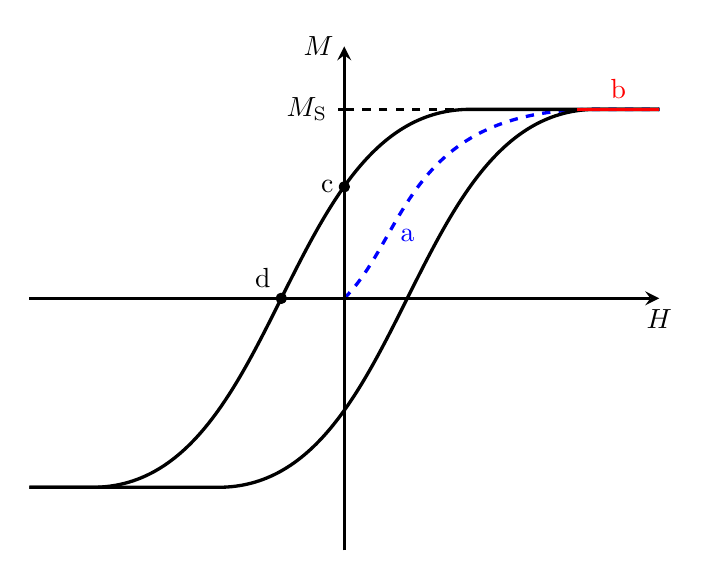
\begin{tikzpicture}[line width = 1.2pt, line join=round,x=1cm,y=1cm,>=stealth, scale = 0.8]
	% Neukurve
	\draw [dashed, color=blue] (0,0) to [controls={+(1,1) and +(-3,0)}] (4,3) -- (5,3);
	% Koordinatensystem
	\draw [->] (-5,0) -- (5,0) node [anchor = north] {$ H $};
	\draw [->] (0,-4) -- (0,4) node [anchor = east] {$ M $};
	% Sättigungs Magnetisierung
	\draw [dashed] (2,3) -- (0,3);
	\draw (0.1,3) -- (-0.1,3) node[anchor=east] {$ M_\mathrm{S} $};
	% Hysteresekurve
	\draw (-5,-3) -- (-4,-3) to [controls={+(3,0) and +(-3,0)}] (2,3) -- (5,3);
	\draw (5,3) -- (4,3) to [controls={+(-3,0) and +(3,0)}] (-2,-3) -- (-5,-3);
	% Erläuterungen
	\draw [color=blue] (1,1) node {a};
	\draw [color=red] (3.7,3) -- (5,3) node [anchor=south,midway] {b};
	\filldraw (0,1.77) circle (1.8pt) node [anchor = east] {c};
	\filldraw (-1,0) circle (1.8pt) node [anchor=south east] {d};
\end{tikzpicture}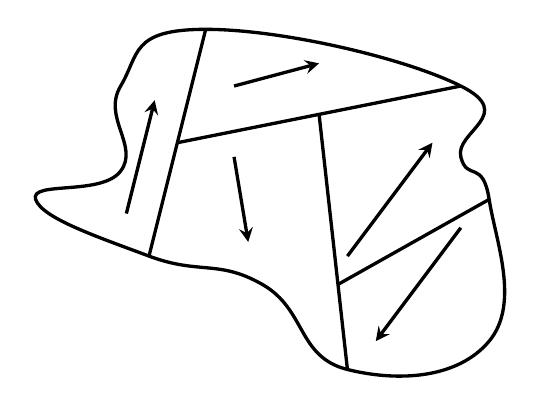
\begin{tikzpicture}[line width = 1.2pt, line join=round,x=0.4cm,y=0.4cm,>=stealth, scale=0.9]
	\coordinate (a) at (0,0);
	\coordinate (b) at (4,-1);
	\coordinate (c) at (7,-4);
	\coordinate (d) at (12,-3);
	\coordinate (e) at (12,2);
	\coordinate (f) at (11,3.5);
	\coordinate (g) at (11,6);
	\coordinate (h) at (2,8);
	\coordinate (i) at (-1,6);
	\coordinate (j) at (-1,3);
	\coordinate (k) at (-4,2);
	% Zwischenpunkte (halbe Strecken meist
	\coordinate (ah) at (1,4);
	\coordinate (ahg) at (6,5);
	% 1/3
	\coordinate (ahgi) at ({6+2/3},-1);
	% Rahmen
	\draw plot [smooth cycle, tension=0.8] coordinates {(a) (b) (c) (d) (e) (f) (g) (h) (i) (j) (k)};
	% Trennlinien
	\draw (a) -- (h);
	\draw (ah) -- (g);
	\draw (ahg) -- (c);
	\draw (ahgi) -- (e);
	% Pfeile
	\draw [->] (-0.8,1.5) -- ++(1,4);
	\draw [->] (3,6) -- ++(3,0.8);
	\draw [->] (3,3.5) -- ++(0.5,-3);
	\draw [->] (7,0) -- ++(3,4);
	\draw [->] (11,1) -- ++(-3,-4);
\end{tikzpicture}
		  \end{center}
		  \begin{itemize}
		  	\item[a)] \textit{Neumagnetisierungskurve} - Magnetisierung aus einem unmagnetisierten Zustand heraus
		  	\item[b)] \textit{Sättigung} - $M$ vergrößert sich nicht mehr bei wachsendem $H$
		  	\item[c)] \textit{Remanenz} - Magnetisierung, die ohne äußeres Feld bestehen bleibt $\to$ Dauermagnete
		  	\item[d)] \textit{Koerzitivfeldstärke} - Feldstärke die benötigt wird um $M=0$ zu erreichen
		  \end{itemize}
		  
	  \textbf{Ferrimagnetismus:}\\
		Der Festkörper setzt sich hier aus zwei Untergittern zusammen.			         Beide für sich sind jeweils ferromagnetisch. Allerdings ist die jeweilige Magnetisierung nicht gleich und kompensiert sich teilweise.\\\\
	\textbf{Antiferromagnetismus:}\\
				        Antiferromagnetismus ist ein Spezialfall des Ferrimagnetismus. Beide Untergitter sind gleich stark magnetisiert, aber in umgekehrte Richtung.
				         Unterhalb der kritischen \textbf{N{\'e}el-Temperatur} gibt es keine Magnetisierung, oberhalb gibt es Paramagnetismus (aber: $\chi_m=\chi_m(H)$).
 \section{Magnetostatische Probleme und ihre Lösung}\label{magstatlsg}
	    Im einfachsten Fall des linearen, isotropen und homogenen Medium als \textbf{gesamtes} Lösungsvolumen muss \ref{vektorpot} gelöst werden. Ebenso kann in \textbf{bereichsweise} linearen, isotropen und homogenen Medien eine Lösung in jedem Teilbereich erfolgen. Die freien Konstanten müssen dann so angepasst werden, dass Stetigkeitsbedingungen nicht verletzt sind.\\
	   Gibt es keine Ströme im Lösungsvolumen $V$ aber Randwerte auf der Oberfläche $O(V)$, dann gilt im Volumen nach \ref{GGms1} $\rot \vec{H}  = \vec{0}$. Daraus folgt, dass $H$ in diesem Fall als Gradientenfeld aufgefasst werden kann ($\nearrow$\ref{poin1}). Also gilt mit dem \textbf{magnetischen Skalarpotential} $\phi_m$:
		              \begin{equation} \label{skalarpotms}
			              \vec{H} (\vec{r} ) = -\grad \phi_m (\vec{r} ) 
		              \end{equation}
		    Bei zumindest bereichsweise konstantem $\mu_r$ folgt ($\nearrow$\ref{GGms2}):
		              \begin{equation}
			              \div \vec{B}  = 0 = \div \left[\mu_0\mu_r \left(-\grad \phi_m \right)\right] \Rightarrow \boxed{\Delta \phi_m = 0}
		              \end{equation}
		         Es handelt sich um eine Laplace-Gleichung. Nun sind aus der Elektrostatik bekannte Lösungsmethoden unter Berücksichtigung der vorgegebenen Randbedingungen anzuwenden ($\nearrow$\ref{pdgl},\ref{poilsg}).\\
	   Gibt es keine Ströme im Lösungsvolumen $V$ aber Randwerte auf der Oberfläche $O(V)$ und \textbf{zusätzlich} eine Magnetisierung $\vec{M}(\vec{r} )\ne \vec{0}$ in $V$, dann gilt \ref{skalarpotms}
		         Mit zumindest bereichsweise konstanten $\mu_r$ folgt ($\nearrow$\ref{GGms2}):
		              \begin{equation}
			              \div \vec{B}  = 0 = \mu_0\div ( \underbrace{-\grad \phi_m }_{\vec{H} }+\vec{M}) \Rightarrow \boxed{\Delta \phi_m = \div \vec{M}} 
		              \end{equation}
		         Es handelt sich um eine Poisson-Gleichung. Ohne Randbedingungen folgt damit analog zu \ref{PotR}:
		              \begin{equation}
			              \phi_m (\vec{r} ) = -\frac{1}{4\pi} \int \frac{\div \vec{M} (\vec{r}' ) }{|\vec{r} -\vec{r}' |} \dd V'
		              \end{equation}
		         Mit Dirichlet- oder Neumann-Randbedingungen sind aus der Elektrostatik bekannte Lösungsmethoden unter Berücksichtigung der vorgegebenen Randbedingungen anzuwenden ($\nearrow$\ref{pdgl},\ref{poilsg}).

